\documentclass[./main.tex]{subfiles}
\begin{document}
\ifSubfilesClassLoaded{\mainmatter}{}

\chapter{Graphical representation} \label{chap:p2c5}

So far we have seen essentially an abstract theory about (pseudo-)metric spaces. This work would not be complete without addressing the relevance of this theory with respect to the problem of phylogenetic reconstruction, as outlined in the \autoref{chap:intro}.

So we are going to make an informal discussion of the connections, stating the principal results without proof.

The content of this chapter is mainly based on \cite{HRS11}. \\
We will assume familiarity with some basics notions and terminology from graph theory. \\
In the following we will use distance function basically as a synonym for dissimilarity function.\bigskip


\subsection*{Basic definitions}

Phylogenetics is the study of the evolutionary history and relationships among or within groups of organisms. \\
The goal of phylogenetic inference is to produce a diagram that represents an \emph{hypothesis} of relationships that reflects the evolutionary history of a group of organisms.

Biologists call \textbf{taxon} (plural \textbf{taxa}) the taxonomic unit that represents some species/group/individual organism whose evolutionary history is of interest.

So in this context $X$ is a (necessarily finite) set of taxa.\bigskip


\subsection*{Phylogenetic trees}

An (unrooted)\footnotemark\ \textbf{phylogenetic tree} is a (graph-theoretical) tree, in which all nodes have degree $\neq 2 \,$, together with a labeling that assigns exactly one taxon to every leaf, and none to any internal node.

\footnotetext{
    From the point of view of phylogenetics it would be more desirable to have \emph{rooted} trees, since they give an explicit direction of time (namely from the root to the leaves); but from a theoretical and algorithmic point of view unrooted trees are easier to work with.
}

\begin{figure}[h]
    \frame{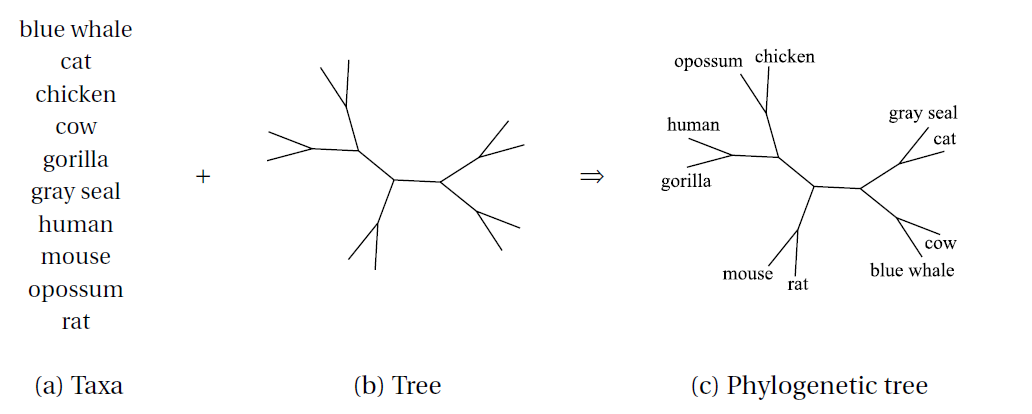
\includegraphics[width=\textwidth]{phylo-tree}}
    \source{\cites[Figure 3.2]{HRS11}}
\end{figure}

In order to quantify the effect of evolution, we assign to each edge a \textbf{weight} or \textbf{length}.\footnotemark

\footnotetext{This number often is proportional to the estimated number of mutations occurred along the edge or is correlated to evolutionary time in some other way.}

A weighted phylogenetic tree $T$ induces a \textbf{tree distance} $D_T$ on each pair of taxa given by the length of the unique path between the leaves labeled by those taxa. Notice that this distance is actually a metric.

We say that a distance function $D$ is an \textbf{additive distance} (or \textbf{tree-like}) \\
\bsp if there exists a phylogenetic tree $T$ such that $\, D = D_T \,$.

A characterization of tree metrics is given in \cite{Bun74}:
\begin{remarklike}[Fact]
    A distance function is additive if and only if \\
    \bsp it satisfies the four-point condition.
\end{remarklike}

\clearpage


\subsection*{Trees and splits}

Any edge of a phylogenetic tree defines a split of the underlying taxon set $X$: deleting the edge produces two subtrees, and their taxon labels constitute the two parts of the split. \\
In fact, since every leaf in a phylogenetic tree is labeled by some taxon, the two parts are non-empty (the two subtrees must contain some leaves); and, since each taxon occurs precisely once, it follows that the two parts are disjoint and cover all the taxa.

If the edges of the tree have lengths/weights, then these can be assigned to the corresponding split.

The \textbf{split encoding} of an (unrooted) phylogenetic tree is the set of all the splits represented by its edges.

\begin{figure}[h]
    \centering
    \frame{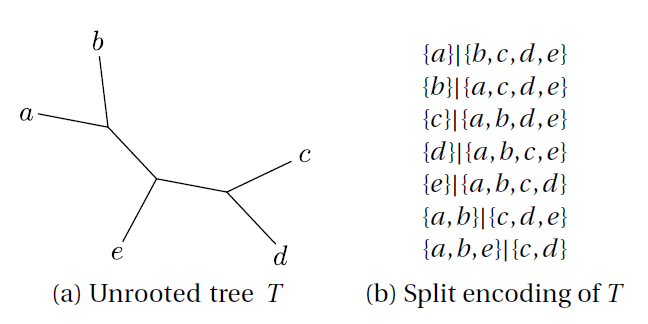
\includegraphics[height=6cm]{splits}}
    \source{\cites[Figure 5.2]{HRS11}}
\end{figure}

\begin{remarklike}[Fact]
    A tree can be uniquely reconstructed from its split encoding.
\end{remarklike}

Thus we can say that a tree $T$ \textbf{represents} (or \textbf{realizes}) a set of splits $\Sc$ \\
\bsp if and only if $\Sc$ coincide with the split encoding of $T$.\bigskip

A classical result by Buneman \cite{Bun72} gives us a characterization of the set of splits induced by a tree.

\begin{remarklike}[Fact]
    Let $\Sc$ be a set of splits on $X$ that contains all trivial splits on $X$.
    
    Then there exists a unique unrooted phylogenetic tree $T$ that represents $\Sc$ if and only if $\Sc$ is compatible.
\end{remarklike}

\clearpage


\subsection*{Split decomposition}

We have defined splits for distances and splits for trees. \\
Now the non-trivial fact to prove is that the split encoding of a tree coincides with the splits of the induced tree metric, and the edge weights coincide with the isolation indices.

\begin{fact}
    Let $d$ be a tree metric. 
    
    Then a split $\{A,B\}$ is a $d$-split if and only if \\[2pt]
    for every $\, a,a^\prime \in A \,$ and $\, b,b^\prime \in B \,$
    \[ a a^\prime + b b^\prime < a b + a^\prime b^\prime = a b^\prime + a^\prime b \nospblw \]

    In this case the split corresponds to a unique edge of length $\aAB$ in the tree representing $d$.
\end{fact}

\begin{proposition}
    If $d$ is a pseudo-metric satisfying the four-point condition, \\
    \bsp then it can be written as
    \[ d = \sum_{S \,\in\, \Sc_d(X)} \alpha_S^d \cdot \delta_S \nospblw \]
    
    Moreover, a collection of splits $\Sc$ is of the form $\Sc = \Sc_d(X)$, \\
    \bsp where $d$ is a pseudo-metric satisfying the four-point condition, \\
    if and only if $\Sc$ is compatible.
\end{proposition}
\begin{proof}
    The first assertion is a consequence of \autoref{teo:teo2} and \autoref{cor:cor7}.

    ($\Rightarrow$) It is a consequence of \autoref{cor:cor7}.

    ($\Leftarrow$) Since compatible implies weakly compatible, \\
    \Bsp{\qquad} it is a consequence of \autoref{teo:teo3} and \autoref{cor:cor7}.
\end{proof}

In other words, tree metrics are totally decomposable, and a collection of splits coincide with the $d$-splits of some tree metric if and only if they are compatible.

\clearpage

In \autoref{prop:4totd} we have seen that pseudo-metrics on $4$ elements are totally decomposable, but their $d$-splits are not necessarily compatible. \\
Thus, in general, they cannot be always represented as trees. \\
However they can be represented as networks where parallel edges correspond to the same split.

\begin{figure}[h]
    \centering
    \frame{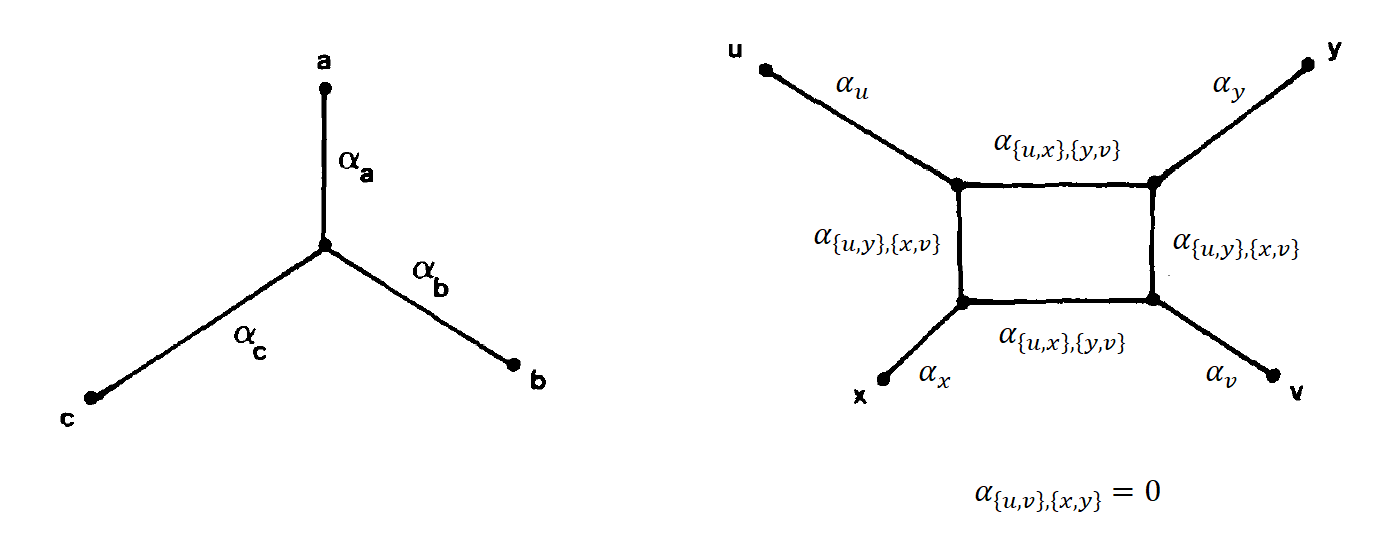
\includegraphics[width=\textwidth]{iso-index}}
    \source{adapted from \cite{BD92a}}
\end{figure}

These observations motivate us to discard the residue also in the general case, and focus only on the totally decomposable part. Our hope is that we can build similar networks that approximate the original distance function.

\clearpage


\subsection*{Split networks}

What kind of networks we are talking about exactly? \\
We want something akin to phylogenetic trees, that can be built from splits.

The precise definition is quite involved but the idea is that each split is represented by one or multiple edges (usually drawn parallel to each other) with the property that removing the edges corresponding to the same split produces exactly two connected components. \\
Such networks are called \textbf{split networks}.\footnotemark

\begin{figure}[h]
    \centering
    \frame{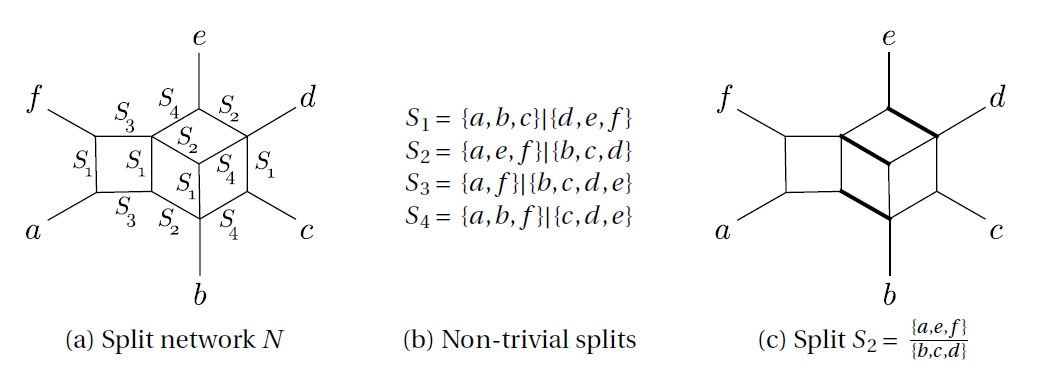
\includegraphics[width=\textwidth]{split-network}}
    \source{\cites[Figure 5.6]{HRS11}}
\end{figure}

\footnotetext{
    The attentive reader may ask why not use the name \emph{phylogenetic networks}. \\
    The reason is there are various different kinds of networks employed in phylogenetics, \\
    \bsp and also there is not much consensus on the terminology \cites[§4.2]{HRS11}.
}

The remarkable result is that a generic collection of splits can always be represented by a split network \cites[§5.6]{HRS11}.
\begin{remarklike}[Fact]
    For any set of splits $\Sc$ there exists a unique split network that represents $\Sc$, called the \textbf{canonical split network} or \\
    \bsp \textbf{Buneman graph} associated with $\Sc$.
\end{remarklike}

There are algorithms that take in input a set of splits and give in output a split network that represents those splits. In particular, the network computed by the convex hull algorithm is the Buneman graph.

\clearpage


\subsection*{The methods}

In this framework the role of split decomposition is to give a collection of splits with certain properties, namely weak compatibility. 

This is a nice property because the split networks associated with weakly compatible splits are often quite close to being planar, as they usually have only a few edges crossing over each other and do not contain any \squote{high-dimensional cubes}, which may occur for completely unrestricted sets of splits.

One of the strength and limitation of the split decomposition method is that it produces relatively few splits. \\
In fact, as the number of taxa increases, also the probability that isolation indices are $0$ increases (it just takes one of the $\beta$ indices to be $0$); as a consequence the number of $d$-splits becomes very contained.

It makes sense to ask: what are the maximal sets of weakly compatible splits? The answer is circular splits.

A set of splits is called \textbf{circular} if the taxa can be placed around a circle in such a way that each split can be realized by a line through the circle; this line separates the plane into two half-planes corresponding to the two parts of the split.

Circular split have a very nice property:
\begin{remarklike}[Fact]
    A set of splits is circular if and only if it can be represented as an outer-labeled planar split network.
\end{remarklike}

\begin{figure}[h]
    \centering
    \frame{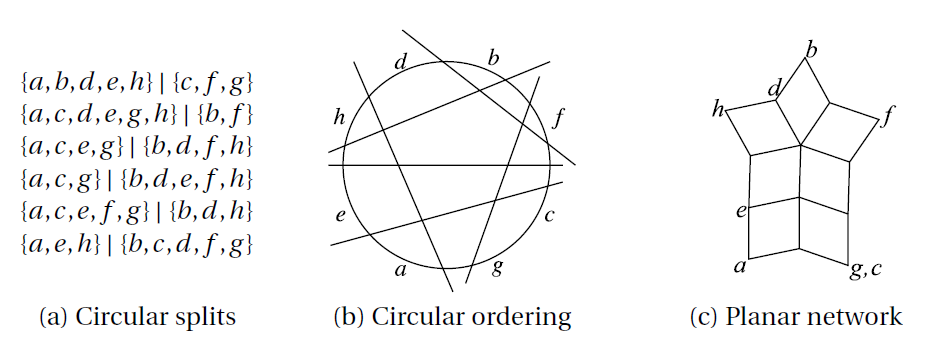
\includegraphics[width=0.95\textwidth]{circular}}
    \source{\cites[Figure 5.9]{HRS11}}
\end{figure}

\clearpage

A successor of the split decomposition method, called NeighborNet \cite{BM04,BH23}, produces a collection of weighted circular splits.\bigskip

\begin{displayquote}[\textup{\cites[§10.4.5]{HRS11}}][]
    Neighbor-net is an attractive method for computing split networks for the following reasons: First, the resulting networks are outer-labeled planar and thus easy to draw and to read. Secondly, the algorithm is quite fast. Thirdly, it produces resolved networks even for quite large numbers of taxa, unlike the split decomposition method, which rapidly loses resolution as the number of taxa increases.
\end{displayquote}

Both methods have the nice property that they produce a tree when given tree-like data.

\end{document}